Efficient execution of parameter-at-a-time queries has been a subject extensively studied in the area of database systems in the past  \cite{selinger:1979aa} \cite{dayal:1987aa} \cite{kim:1982aa} \cite{ganski:1987aa} \cite{seshadri:1996aa}. The first paper to show execution of parameter-at-a-time queries was by Selinger  \cite{selinger:1979aa}. In this setting, only the database is considered, there is no application program holding application-resident data, thus in this context \texttt{SelectedNations} is a database relation. Our running example can be then expressed as shown in figure \ref{fig:taat}. This query is then parsed and compiled into a logical query execution plan, which describes how the query can be executed. 

\begin{figure}[h]
\centering
\begin{minipage}{0.45\textwidth}
\centering
\begin{SQL}
SELECT sn.name, (
   SELECT sum(o.total_price) as sumTotal
    FROM Orders o, Customers c
    WHERE o.cust_ref = c.cust_key
    AND c.nation_ref = sn.nation_key
  ) as sumTotal
 FROM SelectedNations sn
\end{SQL}
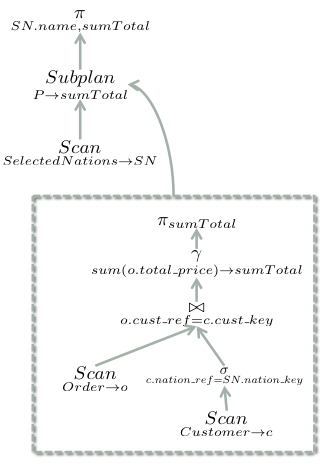
\includegraphics[width=6cm]{images/TAATExecution}
\caption{Parameter-at-a-time Query and Execution}
\label{fig:taat}
\end{minipage} \hfill
\begin{minipage}{0.45\textwidth}
\centering
\begin{SQL}
SELECT SN.name, sum(O.total_price) as sumTotal
FROM SelectedNations SN
LEFT JOIN (Customers C
   JOIN Orders O 
   ON O.cust_ref = C.cust_key)
ON C.nation_ref = SN.nation_key
GROUP BY SN.nation_key, SN.name;
\end{SQL}
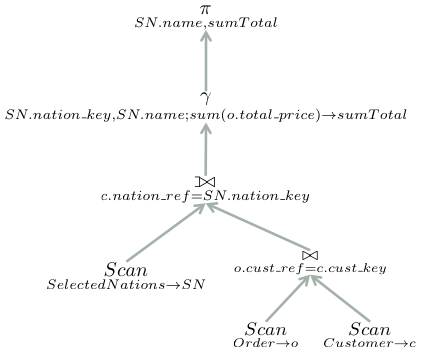
\includegraphics[width=7cm]{images/SAATExecution}
\caption{Set-at-a-time Query and Execution Plan}
\label{fig:saat}
\end{minipage}
\end{figure}

In this execution plan, the subplan operator executes the target query for every selected nation tuple. In each subplan execution, the value \texttt{SN.nation\_key} is parameterized with the value \texttt{nation\_key} column for the \texttt{SN} tuple currently in context. In Selinger's work, this execution plan is followed literally: only the operators within the subplan's inner block are optimized.

Kim \cite{kim:1982aa} was the first to notice that a better evaluation plan was available for such queries, by evaluating all subplans at once, then joining back the result with the outer query. His technique, however, has a bug was discovered by Kiessling \cite{kiessling:1984aa}. The bug was fixed with Dayal's method which introduced the left outer join operator. Dayal's rewriting is shown on figure \ref{fig:saat}. If a selected nation did not have any corresponding customers, Kim's algorithm will not be equivalent to the original plan, while Dayal's algorithm (and all it's successors) do.

Note that Dayal's method can be further optimized by joining a copy of distinct \texttt{SelectedNations} with \texttt{Customers} before the join with \texttt{Orders}. This is the approach taken by Seshadri \cite{seshadri:1996aa}, dubbed \emph{Magic Decorrelation}, which provides a more efficient kind of execution. Even if the number of selected nations is very small, Magic decorrelation (plan on figure \ref{fig:magic}) ensures that only those customers from qualifying nations are fetched, and no more than once.

\begin{figure*}[h]
\begin{minipage}{0.45\textwidth}
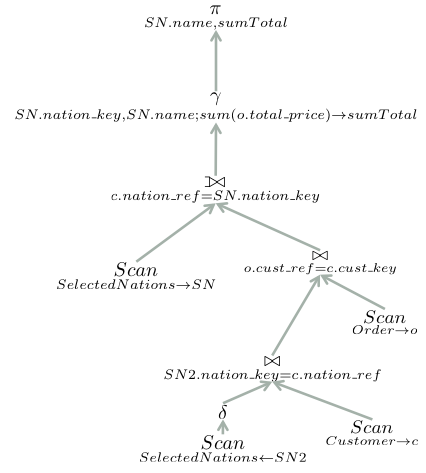
\includegraphics[width=7cm]{images/MagicDecorrelation}
\caption{Magic Decorrelation Execution Plan}
\label{fig:magic}\hfill
\end{minipage}
\begin{minipage}{0.45\textwidth}
\centering
\begin{Java}[basicstyle=\small]
public List getSumTotals(List selectedNations) {
List sumTotals = new ArrayList();
PreparedStatement stmt = conn.prepareStatement( "SELECT sum(o.total_price) as sumTotal "
       + "FROM Orders o, Customers c "
       + "WHERE o.cust_ref = c.cust_key "
       + "AND c.nation_ref = ?");
LoopContextTable lct = new LCT();
int key = nation.getKey();
for (Nation nation : selectedNations) {
    LoopContext ctx= lct.createContext();
    stmt.setInt(1, key);
    ctx.setInt("nation", key);
    stmt.addBatch(ctx);
}
stmt.executeBatch();
for (LoopContext ctx : lct) {
    ResultSet rs = stmt.getResultSet(ctx);
    rs.next();
    int sum = rs.getInt("sum");
    sumTotals.add(Pair.of(nation, sum));
}
return sumTotals;
}
\end{Java}
\caption{Loop Fission}
\label{fig:loopfission}
\end{minipage}
\end{figure*}

Execution plans on figures \ref{fig:saat} and \ref{fig:taat} are semantically equivalent, and the database optimizer can choose either execution to answer the running example query. Which execution plan is the most efficient relies on a number of factors: when the selected nations is very small (just a single nation is selected), the parameter-at-a-time method is actually slightly faster, because fewer operators are used and the subplan is only executed once. As soon as the number of selected nations increases, the magic decorrelation outperforms the parameter at a time execution significantly. That being said, some parameter-at-a-time executions (for example queries with set operators) cannot be rewritten \cite{pirahesh:1992aa} using query decorrelation. However, other techniques are possible, such as caching portions of the subplan which aren't accessed using outer references \cite{rao:1998aa}, since the data they represent do not change between subplan iterations.

Back in the context of web applications, set-at-time execution has the added benefit in web applications to minimize network round-trip delays (only one round-trip is required, no matter how many nations are selected) and  maximizing bandwidth throughput (all the data comes back at once). It can also be applied directly by the programmer, as one can see on figure \ref{fig:code2} (see appendix). In this code fragment, the magic decorrelation evaluation plan is transcribed by the programmer directly in SQL on lines 6-15, while the selected nation keys are added to the SQL query as strings (line 4).

Unfortunately, manually writing a set-at-a-time execution program is cumbersome and error prone. The techniques that we discuss in the next section attempt to solve this problem by allowing programmers to write programs using parameter-at-a-time formulation but have them execute like a set-at-a-time formulation.






